\documentclass{article}[a4paper]

\usepackage[fleqn]{amsmath} % This package with the fleqn option aligns equations to the left
\setlength{\mathindent}{0pt} % Set indentation from the left margin

\usepackage{amssymb} % Required for math symbols
\usepackage{graphicx} % Required for inserting images
\usepackage{geometry}

\usepackage{float} % Use this package to control float behavior

\usepackage{algorithm}
\usepackage{algpseudocode}

\usepackage[backend=biber, style=authoryear, citestyle=authoryear]{biblatex}
\addbibresource{references.bib}

\geometry{a4paper, margin=1in}

{
\title{
    
\includegraphics[width=0.34\textwidth]{/Users/mlnick/documents/images/tsukuba-logo.png} \\
    \vspace{2mm}
    \textbf{Numerical Simulation} \\
    \vspace{3mm}    
    Project 2 \\
    Finite Difference Time Domain Simulation
}

\author{Mamanchuk Mykola, SID.202420671}
% \date{\today}
\date{\today}
}

\usepackage{listings}
\usepackage{color}

\definecolor{codegreen}{rgb}{0,0.6,0}
\definecolor{codegray}{rgb}{0.5,0.5,0.5}
\definecolor{codepurple}{rgb}{0.58,0,0.82}
\definecolor{backcolour}{rgb}{0.99,0.99,0.99}

\lstdefinestyle{mystyle}{
    backgroundcolor=\color{backcolour},   
    commentstyle=\color{codegreen},
    keywordstyle=\color{magenta},
    numberstyle=\tiny\color{codegray},
    stringstyle=\color{codepurple},
    basicstyle=\ttfamily\footnotesize,
    breakatwhitespace=false,         
    breaklines=true,                 
    captionpos=b,                    
    keepspaces=true,                 
    numbers=left,                    
    numbersep=5pt,                  
    showspaces=false,                
    showstringspaces=false,
    showtabs=false,                  
    tabsize=2
}
\lstset{style=mystyle}

\begin{document}

\maketitle

\section{Introduction}

\subsection{Project Overview}
This project focuses on the implementation of the one-dimensional Finite Difference Time Domain (1D FDTD) method. The FDTD method is widely used in computational electromagnetics to simulate the propagation of electromagnetic waves through various media. By discretizing Maxwell's equations in both time and space, it provides a dynamic visualization of wave behavior, which is crucial for understanding and designing electromagnetic systems.

\subsection{Objectives}
The primary objectives of this project are:
\begin{itemize}
    \item To develop a Python program that implements the 1D FDTD method with periodic boundary conditions.
    \item To investigate the propagation characteristics of an electromagnetic wave initiated by a discrete impulse at the center of the computational domain.
    \item To analyze the impact of boundary conditions and grid resolution on the simulation results.
\end{itemize}

\subsection{Significance}
The significance of the FDTD method lies in its ability to model complex electromagnetic phenomena with high accuracy. This project not only serves as an educational tool to understand the basic principles of wave propagation but also provides a foundation for more advanced studies in electromagnetic wave interactions with various materials and structures.

\section{Theory Related Essentials}

The FDTD method is a numerical analysis technique used for modeling computational electrodynamics (finding approximate solutions to the associated system of differential equations). Since it is a time-domain method, solutions can cover a wide range of frequencies with a single simulation run.

\subsection{Maxwell's Equations}
The FDTD method is based on Maxwell's equations, which describe how electric and magnetic fields are generated and altered by each other as well as by charges and currents. These equations are both the foundation and the ultimate test for any electromagnetic simulation method.

\subsection{Discretization}
The core idea behind FDTD is to use a discrete grid spatially (in one, two, or three dimensions) and a discrete time step. Each field component in Maxwell's equations is updated in time with finite differences that approximate the derivatives. The Yee grid, a staggered grid, helps in the implementation of the FDTD by storing electric and magnetic field components at different points in the grid, which avoids numerical instabilities and ensures the fields are updated accurately.

\subsection{Numerical Stability and Dispersion}
Numerical stability is achieved by satisfying the CFL condition, which provides a criterion for the selection of a stable time-step based on the spatial discretization and the speed of light in the medium. Numerical dispersion, an artifact of the discretization of the continuous wave equations, can affect the accuracy of the wave propagation in the numerical model and needs to be minimized.

This theoretical framework supports the numerical experiments conducted in this project, where the dynamics of electromagnetic waves in a discretized space-time grid are explored using the FDTD method.

\section{Implementation}

This section details the implementation of the 1D FDTD method for simulating the propagation of electromagnetic waves. The simulation focuses on the evolution of electric and magnetic fields over a discretized space and time.

\subsection{Code Explanation}
The implementation uses NumPy for handling array operations, which represent the electric and magnetic fields across the spatial grid. The Python script performs the following key tasks:
\begin{itemize}
    \item Initializes the computational domain and the electromagnetic field values.
    \item Applies an initial impulse to the electric field at the center of the domain.
    \item Updates the magnetic field based on the spatial derivative of the electric field, using finite differences.
    \item Implements periodic boundary conditions to simulate an infinite domain.
    \item Updates the electric field using the spatial derivative of the magnetic field.
    \item Plots the electric and magnetic field distributions at the final time step.
\end{itemize}

The simulation grid consists of 200 points (variable \texttt{L}), with a normalized spatial step (\texttt{dx = 1.0}) and a time step (\texttt{dt = 0.5}) chosen to satisfy the CFL condition for numerical stability. The simulation runs for a single time step to demonstrate the initial propagation of the fields from the impulse.

\subsection{Pseudocode}

Below you can see the pseudocode realization for the task.

\begin{algorithm}[H]
\caption{1D FDTD Simulation}
\begin{algorithmic}[1]
\State \textbf{Initialize} grid size $L$, time step $dt$, space step $dx$
\State \textbf{Initialize} arrays $Ey$ and $Bz$ with zeros
\State \textbf{Set} $Ey[\frac{L}{2}] \gets 1$ \Comment{Initial impulse}
\For{$n = 0$ to $T-1$}
    \For{$i = 0$ to $L-2$}
        \State $Bz[i] \gets Bz[i] - \frac{dt}{dx} \cdot (Ey[i+1] - Ey[i])$
    \EndFor
    \State $Bz[L-1] \gets Bz[L-1] - \frac{dt}{dx} \cdot (Ey[0] - Ey[L-1])$ \Comment{Periodic boundary}
    \For{$i = 1$ to $L-1$}
        \State $Ey[i] \gets Ey[i] - \frac{dt}{dx} \cdot (Bz[i] - Bz[i-1])$
    \EndFor
    \State $Ey[0] \gets Ey[0] - \frac{dt}{dx} \cdot (Bz[0] - Bz[L-1])$ \Comment{Periodic boundary}
\EndFor
\end{algorithmic}
\end{algorithm}

\subsection{Python Implementation}

The implementation of the program in Python can be reviewed below.

\begin{lstlisting}[language=Python, caption=1D FDTD Simulation in Python]
import numpy as np
import matplotlib.pyplot as plt

# Constants
L = 200  # Number of grid points
dx = 1.0  # Space step, normalized to 1
dt = dx / 2  # Time step, satisfies CFL condition for stability
T = 1  # Number of time steps to simulate
Ey = np.zeros(L)  # Electric field
Bz = np.zeros(L)  # Magnetic field
Ey[L//2] = 1  # Initial impulse in Electric field

# Simulation
for n in range(T):
    Bz[:-1] = Bz[:-1] - (dt/dx) * (Ey[1:] - Ey[:-1])
    Bz[-1] = Bz[-1] - (dt/dx) * (Ey[0] - Ey[-1])  # Periodic boundary condition
    Ey[1:] = Ey[1:] - (dt/dx) * (Bz[1:] - Bz[:-1])
    Ey[0] = Ey[0] - (dt/dx) * (Bz[0] - Bz[-1])  # Periodic boundary condition

# Plotting
plt.figure(figsize=(10, 4))
plt.subplot(1, 2, 1)
plt.plot(np.linspace(0, 1, L), Ey, label='Electric Field (Ey)')
plt.title('Electric Field at Final Time Step')
plt.xlabel('Normalized Grid Position')
plt.ylabel('Field Amplitude')
plt.grid(True)

plt.subplot(1, 2, 2)
plt.plot(np.linspace(0, 1, L), Bz, color='red', label='Magnetic Field (Bz)')
plt.title('Magnetic Field at Final Time Step')
plt.xlabel('Normalized Grid Position')
plt.grid(True)

plt.tight_layout()
plt.show()
\end{lstlisting}

\section{Graphs and Results Showcase}

\subsection{Initial Condition at \( T = 0 \)}
\begin{figure}[H]
    \centering
    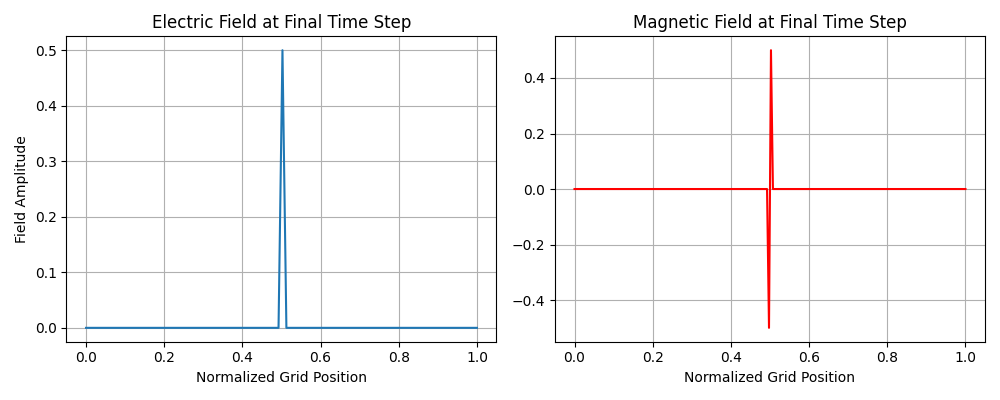
\includegraphics[width=0.8\textwidth]{materials/Figure_0.png}
    \caption{Initial condition showing a single impulse in the electric field \( E_y \) at the center of the grid, and no initial magnetic field \( B_z \). This setup illustrates the starting point for the simulation, demonstrating the localized nature of the initial disturbance.}
\end{figure}

\subsection{Field Evolution at \( T = 25 \)}
\begin{figure}[H]
    \centering
    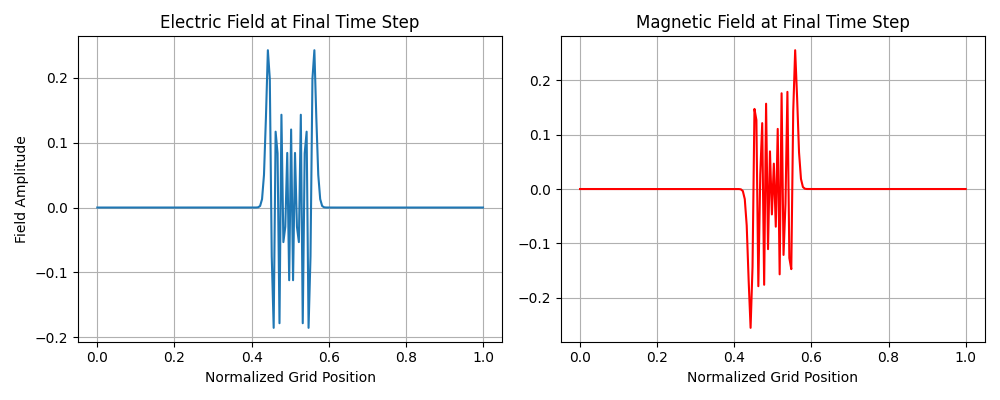
\includegraphics[width=0.8\textwidth]{materials/Figure_25.png}
    \caption{Electric and magnetic fields at \( T = 25 \). The plots show the beginning of wave propagation away from the center, where the initial impulse was applied. The electric field shows minor fluctuations, while the magnetic field begins to show a clear wave pattern as a result of the changing electric field.}
\end{figure}

\subsection{Field Evolution at \( T = 50 \)}
\begin{figure}[H]
    \centering
    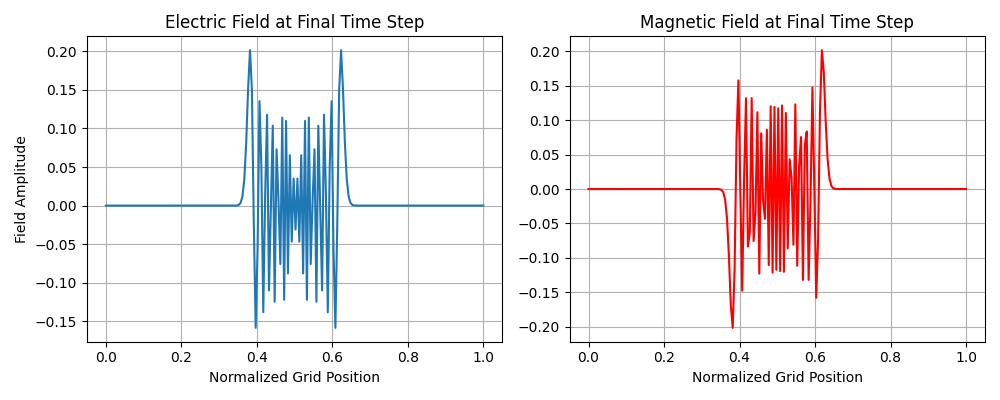
\includegraphics[width=0.8\textwidth]{materials/Figure_50.png}
    \caption{At \( T = 50 \), the fields exhibit more defined wave patterns. The electric field's amplitude starts to increase, demonstrating the effect of periodic boundary conditions that begin to influence the results as the wave reflects back from the boundaries.}
\end{figure}

\subsection{Field Evolution at \( T = 100 \)}
\begin{figure}[H]
    \centering
    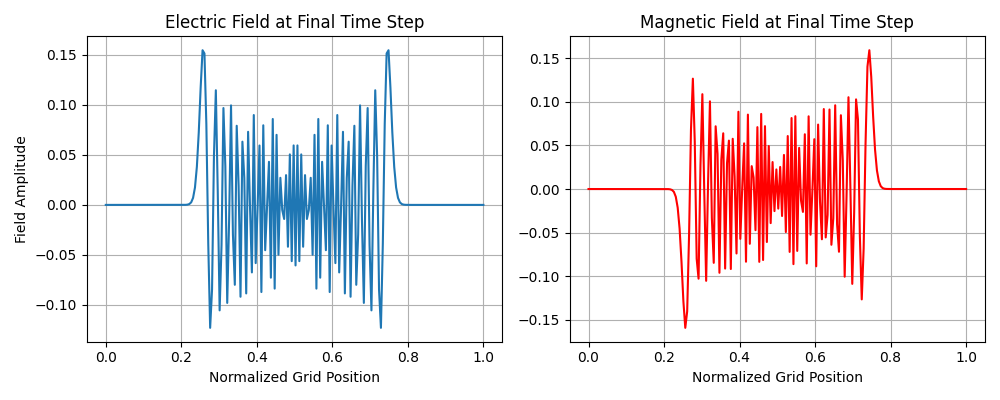
\includegraphics[width=0.8\textwidth]{materials/Figure_100.png}
    \caption{By \( T = 100 \), the wave patterns in both fields are well-established with significant fluctuations. This represents the fully developed wave behavior, including reflections and interference patterns caused by the periodic boundary conditions, illustrating the dynamic evolution of both fields over time.}
\end{figure}

\section{Conclusion}

This project successfully implemented a 1D FDTD simulation to study the evolution of electromagnetic fields over a discretized spatial grid with periodic boundary conditions. The primary objective was to observe the behavior of electric and magnetic fields initiated from a localized impulse at the center of the domain.

The results demonstrated several key aspects of electromagnetic wave propagation:
\begin{itemize}
    \item The initialization of a single impulse in the electric field led to the generation and propagation of both electric and magnetic waves along the grid, confirming the interdependent dynamics described by Maxwell's equations in a discretized space-time framework.
    \item As time progressed, the waveforms exhibited increasing complexity, including reflections and interference patterns due to the periodic boundary conditions. This behavior underscores the significance of boundary conditions in electromagnetic simulations and their impact on the field evolution.
    \item The amplitude and shape of the waves at various time steps provided insights into the wave propagation speed, stability of the simulation under the CFL condition, and the effects of spatial and temporal discretization on the accuracy and physical fidelity of the simulation.
\end{itemize}

Overall, the project not only reinforced the theoretical foundations of electromagnetic wave propagation but also highlighted the practical challenges and considerations in implementing numerical simulations that are crucial for accurate predictions and analyses in computational electrodynamics. Future work could extend this simulation to higher dimensions or explore different initial conditions and boundary configurations to further investigate the diverse phenomena in electromagnetic theory.

\section*{References}
\begin{enumerate}
    \item \textbf{Mamanchuk N., University of Tsukuba}, Github, \today. Available online: \url{https://github.com/RIFLE}
    % \item \textbf{Company}, Name of Work, year. Available online: \url{https://...} [Accessed: yyyy-mm-dd]
\end{enumerate}

\end{document}
